\documentclass[crop,tikz]{standalone}


\usepackage{amsmath,amssymb,amsfonts}
\usepackage{tikz}
\usepackage{pgfplots}
\pgfplotsset{compat=newest}


\usetikzlibrary{shapes, positioning, matrix, calc, pgfplots.statistics, pgfplots.groupplots, pgfplots.colorbrewer, 3d, arrows, positioning, quotes, backgrounds, arrows.meta, spy}

\begin{document}

\begin{tikzpicture}
[   cnode/.style={draw=black,fill=#1,minimum width=3mm,circle},
]

    % Input
    \node[cnode=teal, label={[above, color=teal] $\mathbf{x}_i$}] (x-1) at (0,{-1.8}) {};
    \node[cnode=teal] (x-2) at (0,{-2.8}) {};
    \node[cnode=teal] (x-3) at (0,{-4.2}) {};
    \node at (0,-3.3) {$\vdots$};
    \draw[teal, dashed, rounded corners, thick]
        ($(x-1.north west)+(-0.1cm,0.1cm)$)
        rectangle ($(x-3.south east)+(0.1cm,-0.1cm)$);

    \node[below = 0.2cm of x-3, align=center, text width=1cm, teal] (ls) {input
    layer};

    \matrix (mat_in) [%matrix of math nodes,
        draw, dotted, black, left=1cm of x-2, yshift=-0.2cm,
        label={[below, yshift=-2.9cm] input count matrix $x$},
        %row 1/.style={nodes={font=\small}}
        ]
    {
    & \node[draw=none, font=\tiny] {Gene 1}; & \node[draw=none, font=\tiny]{Gene 2}; &
    \node[draw=none, font=\tiny]{Gene 3}; & \node[draw=none, font=\tiny]{...};\\
    \hline
    %1 & 1 & 1 & 1 &1\\
    \node[draw=none, font=\tiny] (l1l) {Cell 1};   & \node[draw=none, font=\tiny]{0}; & \node[draw=none, font=\tiny]{5}; &
        \node[draw=none, font=\tiny]{29}; & \node[draw=none, font=\tiny] (l1r) {...};  \\
    \node[draw=none, font=\tiny]{Cell 2};   & \node[draw=none, font=\tiny]{0}; & \node[draw=none, font=\tiny]{11}; &
        \node[draw=none, font=\tiny]{13}; & \node[draw=none, font=\tiny]{...};  \\
    \node[draw=none, font=\tiny]{Cell 3};   & \node[draw=none, font=\tiny]{3}; & \node[draw=none, font=\tiny]{0}; &
        \node[draw=none, font=\tiny]{0}; & \node[draw=none, font=\tiny]{...};  \\
    \node[draw=none, font=\tiny]{Cell 4};   & \node[draw=none, font=\tiny]{4}; & \node[draw=none, font=\tiny]{34}; &
        \node[draw=none, font=\tiny]{0}; & \node[draw=none, font=\tiny]{...};  \\
    \node[draw=none, font=\tiny] {...};      & \node[draw=none, font=\tiny]{...}; & \node[draw=none, font=\tiny]{...}; &
        \node[draw=none, font=\tiny]{...}; & \node[draw=none, font=\tiny]{...};  \\
    };
    \draw[teal, dashed, rounded corners, thick]
        ($(l1l.north west)+(-0.0cm,-0.05cm)$)
        rectangle ($(l1r.south east)+(0.1cm,-0.1cm)$);
    \draw[->, teal, thick] ($(l1r)+(-0.3cm,0.3cm)$) to [out=70, in=140]
        ($(x-1)+(-0.3cm,0cm)$);

    % Encoder
    \foreach \x in {1,...,4}
    {   \pgfmathparse{\x<4 ? \x : "n"}

        \node[cnode=gray%,label=90:$l^1_{\pgfmathresult}$
              ] (e-\x) at (1.5,{-\x-div(\x,4)}) {};
        \node[cnode=gray%,label=90:$l^2_{\pgfmathresult}$
              ](e2-\x) at (3,{-\x-div(\x,4)}) {};
    }
    \node at (1.5,-3.7) {$\vdots$};
    \node at (3.0,-3.7) {$\vdots$};

    \node[below = 0.2cm of e-4, xshift=0.75cm, align=center, text width=3cm] (hl)
        {encoder \\ hidden layers};

    \foreach \x in {1,...,3}
    {   \foreach \y in {1,...,4}
        {   \draw[->] (x-\x) -- (e-\y);
        }
    }

    \foreach \x in {1,...,4}
    {   \foreach \y in {1,...,4}
        {
            \draw[->] (e-\x) -- (e2-\y);
        }
    }

    % Latent space
    \node[cnode=orange, label={[above, color=orange] ${\boldsymbol\mu}_i$}] (m-1) at (4.5,{-1.5}) {};
    \node[cnode=orange] (m-2) at (4.5,{-2.5}) {};
    \draw[orange, dashed, rounded corners, thick]
        ($(m-1.north west)+(-0.1cm,0.1cm)$)
        rectangle ($(m-2.south east)+(0.1cm,-0.1cm)$);

    \node[cnode=orange, label={[above, color=orange] ${\boldsymbol\sigma}^2_i$}] (s-1) at (4.5,{-3.5}) {};
    \node[cnode=orange] (s-2) at (4.5,{-4.5}) {};
    \draw[orange, dashed, rounded corners, thick]
        ($(s-1.north west)+(-0.1cm,0.1cm)$)
        rectangle ($(s-2.south east)+(0.1cm,-0.1cm)$);

    \node[right = 0.8cm of m-1, yshift=2.0cm, label={[below, yshift=-2.0cm]
    dimension reduction}] (z_illus) {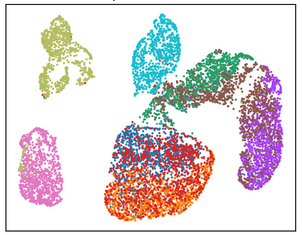
\includegraphics[width=2.5cm]{z.png}};
    \draw[->] ($(m-1)+(0.3cm,-0.5cm)$) to [out=0, in=270]
        ($(z_illus.south)+(0cm,-0.25cm)$);

    \node[cnode=olive, label={[above, color=olive] $\mathbf{z}_i$}] (z-1) at (7.0,{-2.5}) {};
    \node[cnode=olive] (z-2) at (7.0,{-3.5}) {};
    \draw[olive, dashed, rounded corners, thick]
        ($(z-1.north west)+(-0.1cm,0.1cm)$)
        rectangle ($(z-2.south east)+(0.1cm,-0.1cm)$);

    \node[below = 0.2cm of z-2, align=center, text width=1cm, olive] (ls) {latent
    space};

    \draw[->] ($(m-2)+(0.3cm,0cm)$) -- node[below, yshift=-0.22cm] {sample}
        ($(z-1)+(-0.3cm,0cm)$);
    \draw[->] ($(s-1)+(0.3cm,0cm)$) --
        ($(z-2)+(-0.3cm,0cm)$);

    \node at (4.5,-1.8) {$\vdots$};
    \node at (4.5,-3.8) {$\vdots$};
    \node at (7.0,-2.8) {$\vdots$};

    \foreach \x in {1,...,2}
    {   \foreach \y in {1,...,4}
        {
            \draw[->] (e2-\y) -- (m-\x);
            \draw[->] (e2-\y) -- (s-\x);
        }
    }

    % Decoder
    \foreach \x in {1,...,4}
    {   \pgfmathparse{\x<4 ? \x : "n"}

        \node[cnode=gray%,label=90:$l^1_{\pgfmathresult}$
              ] (d-\x) at (8.5,{-\x-div(\x,4)}) {};
        \node[cnode=gray%,label=90:$l^2_{\pgfmathresult}$
              ](d2-\x) at (10.0,{-\x-div(\x,4)}) {};
    }

    \node at (8.5,-3.7) {$\vdots$};
    \node at (10.0,-3.7) {$\vdots$};
    \node[below = 0.2cm of d-4, xshift=0.75cm, align=center, text width=3cm] (dl)
        {decoder \\ hidden layers};

    \foreach \z in {1,...,2}
    {   \foreach \y in {1,...,4}
        {   \draw[->] (z-\z) -- (d-\y);
        }
    }

    \foreach \x in {1,...,4}
    {   \foreach \y in {1,...,4}
        {
            \draw[->] (d-\x) -- (d2-\y);
        }
    }

    % Output
    \node[cnode=teal, label={[above, color=teal] $\hat{\mathbf{x}}_i$}] (x_-1) at (11.5,{-1.8}) {};
    \node[cnode=teal] (x_-2) at (11.5,{-2.8}) {};
    \node[cnode=teal] (x_-3) at (11.5,{-4.2}) {};
    \node at (11.5,-3.3) {$\vdots$};
    \draw[teal, dashed, rounded corners, thick]
        ($(x_-1.north west)+(-0.1cm,0.1cm)$)
        rectangle ($(x_-3.south east)+(0.1cm,-0.1cm)$);
    \node[below = 0.2cm of x_-3, align=center, text width=1cm, teal] (ls)
    {output layer};

    \foreach \x in {1,...,3}
    {   \foreach \y in {1,...,4}
        {   \draw[->] (d2-\y) -- (x_-\x);
        }
    }

    \matrix (mat_out) [draw, dotted, black, right=1cm of x_-2, yshift=-0.2cm,
        label={[below, yshift=-2.9cm] reconstructed count matrix $\hat{x}$}]
    {
    & \node[draw=none, font=\tiny] {Gene 1}; & \node[draw=none, font=\tiny]{Gene 2}; &
    \node[draw=none, font=\tiny]{Gene 3}; & \node[draw=none, font=\tiny]{...};\\
    \hline
    %1 & 1 & 1 & 1 &1\\
    \node[draw=none, font=\tiny] (l1l_) {Cell 1};   & \node[draw=none, font=\tiny]{0}; & \node[draw=none, font=\tiny]{5}; &
        \node[draw=none, font=\tiny]{29}; & \node[draw=none, font=\tiny] (l1r_) {...};  \\
    \node[draw=none, font=\tiny]{Cell 2};   & \node[draw=none, font=\tiny]{0}; & \node[draw=none, font=\tiny]{11}; &
        \node[draw=none, font=\tiny]{13}; & \node[draw=none, font=\tiny]{...};  \\
    \node[draw=none, font=\tiny]{Cell 3};   & \node[draw=none, font=\tiny]{3}; & \node[draw=none, font=\tiny]{0}; &
        \node[draw=none, font=\tiny]{0}; & \node[draw=none, font=\tiny]{...};  \\
    \node[draw=none, font=\tiny]{Cell 4};   & \node[draw=none, font=\tiny]{4}; & \node[draw=none, font=\tiny]{34}; &
        \node[draw=none, font=\tiny]{0}; & \node[draw=none, font=\tiny]{...};  \\
    \node[draw=none, font=\tiny] {...};      & \node[draw=none, font=\tiny]{...}; & \node[draw=none, font=\tiny]{...}; &
        \node[draw=none, font=\tiny]{...}; & \node[draw=none, font=\tiny]{...};  \\
    };
    \draw[teal, dashed, rounded corners, thick]
        ($(l1l_.north west)+(-0cm,-0.05cm)$)
        rectangle ($(l1r_.south east)+(0.1cm,-0.1cm)$);
    \draw[->, teal, thick] ($(x_-1)+(0.3cm,0.0cm)$) to [out=00, in=140]
        ($(l1l_.north west)+(-0.0cm,0cm)$);
    %\foreach \x in {1,...,3}
    %{
    %    \draw[->] (l-\x) -- node[black,above,sloped,pos=0.3] {$\gamma_{\x}$} (s);
    %}

    %\foreach \x in {1,...,3}
    %{   \foreach \y in {1,...,4}
    %    {
    %        \draw[->] (p2-\y) -- (l-\x);
    %    }
    %}

    %\draw [decorate, decoration={brace, mirror, amplitude=5pt}] ($(p-4)+(-1.5,-0.3)$) -- ($(p2-4)+(1.45,-0.3)$) node [below, black, midway, yshift=-0.1cm] {unconstrained part};
    %\draw [decorate, decoration={brace, mirror, amplitude=5pt}] ($(p2-4)+(1.55,-0.3)$) -- ($(p2-4)+(3,-0.3)$) node [below, black, midway, yshift=-0.1cm] {constrained part};
\end{tikzpicture}

\end{document}
